\newpage
\subsection{Расчет заработной платы}
%\todo{ÏÈÑÀÒÜ}

% Бригадир ведет табели учета рабочего времени (рис. \ref{pic:f44}).


Для расчета заработной платы и автоматизации функций управления персоналом используется система 1С: УПП.

%Для расчета рабочего времени персонала используется табели из электронной проходной на базе платформы 1С: Предприятие.
На гофроагрегате и линиях переработки используется сдельная система оплаты труда. Мастера формируют табеля учета рабочего времени и наряды по производственному персоналу в системе 1С: УПП.

\clearpage

%\newpage
%\begin{figure}
%\begin{center}
 %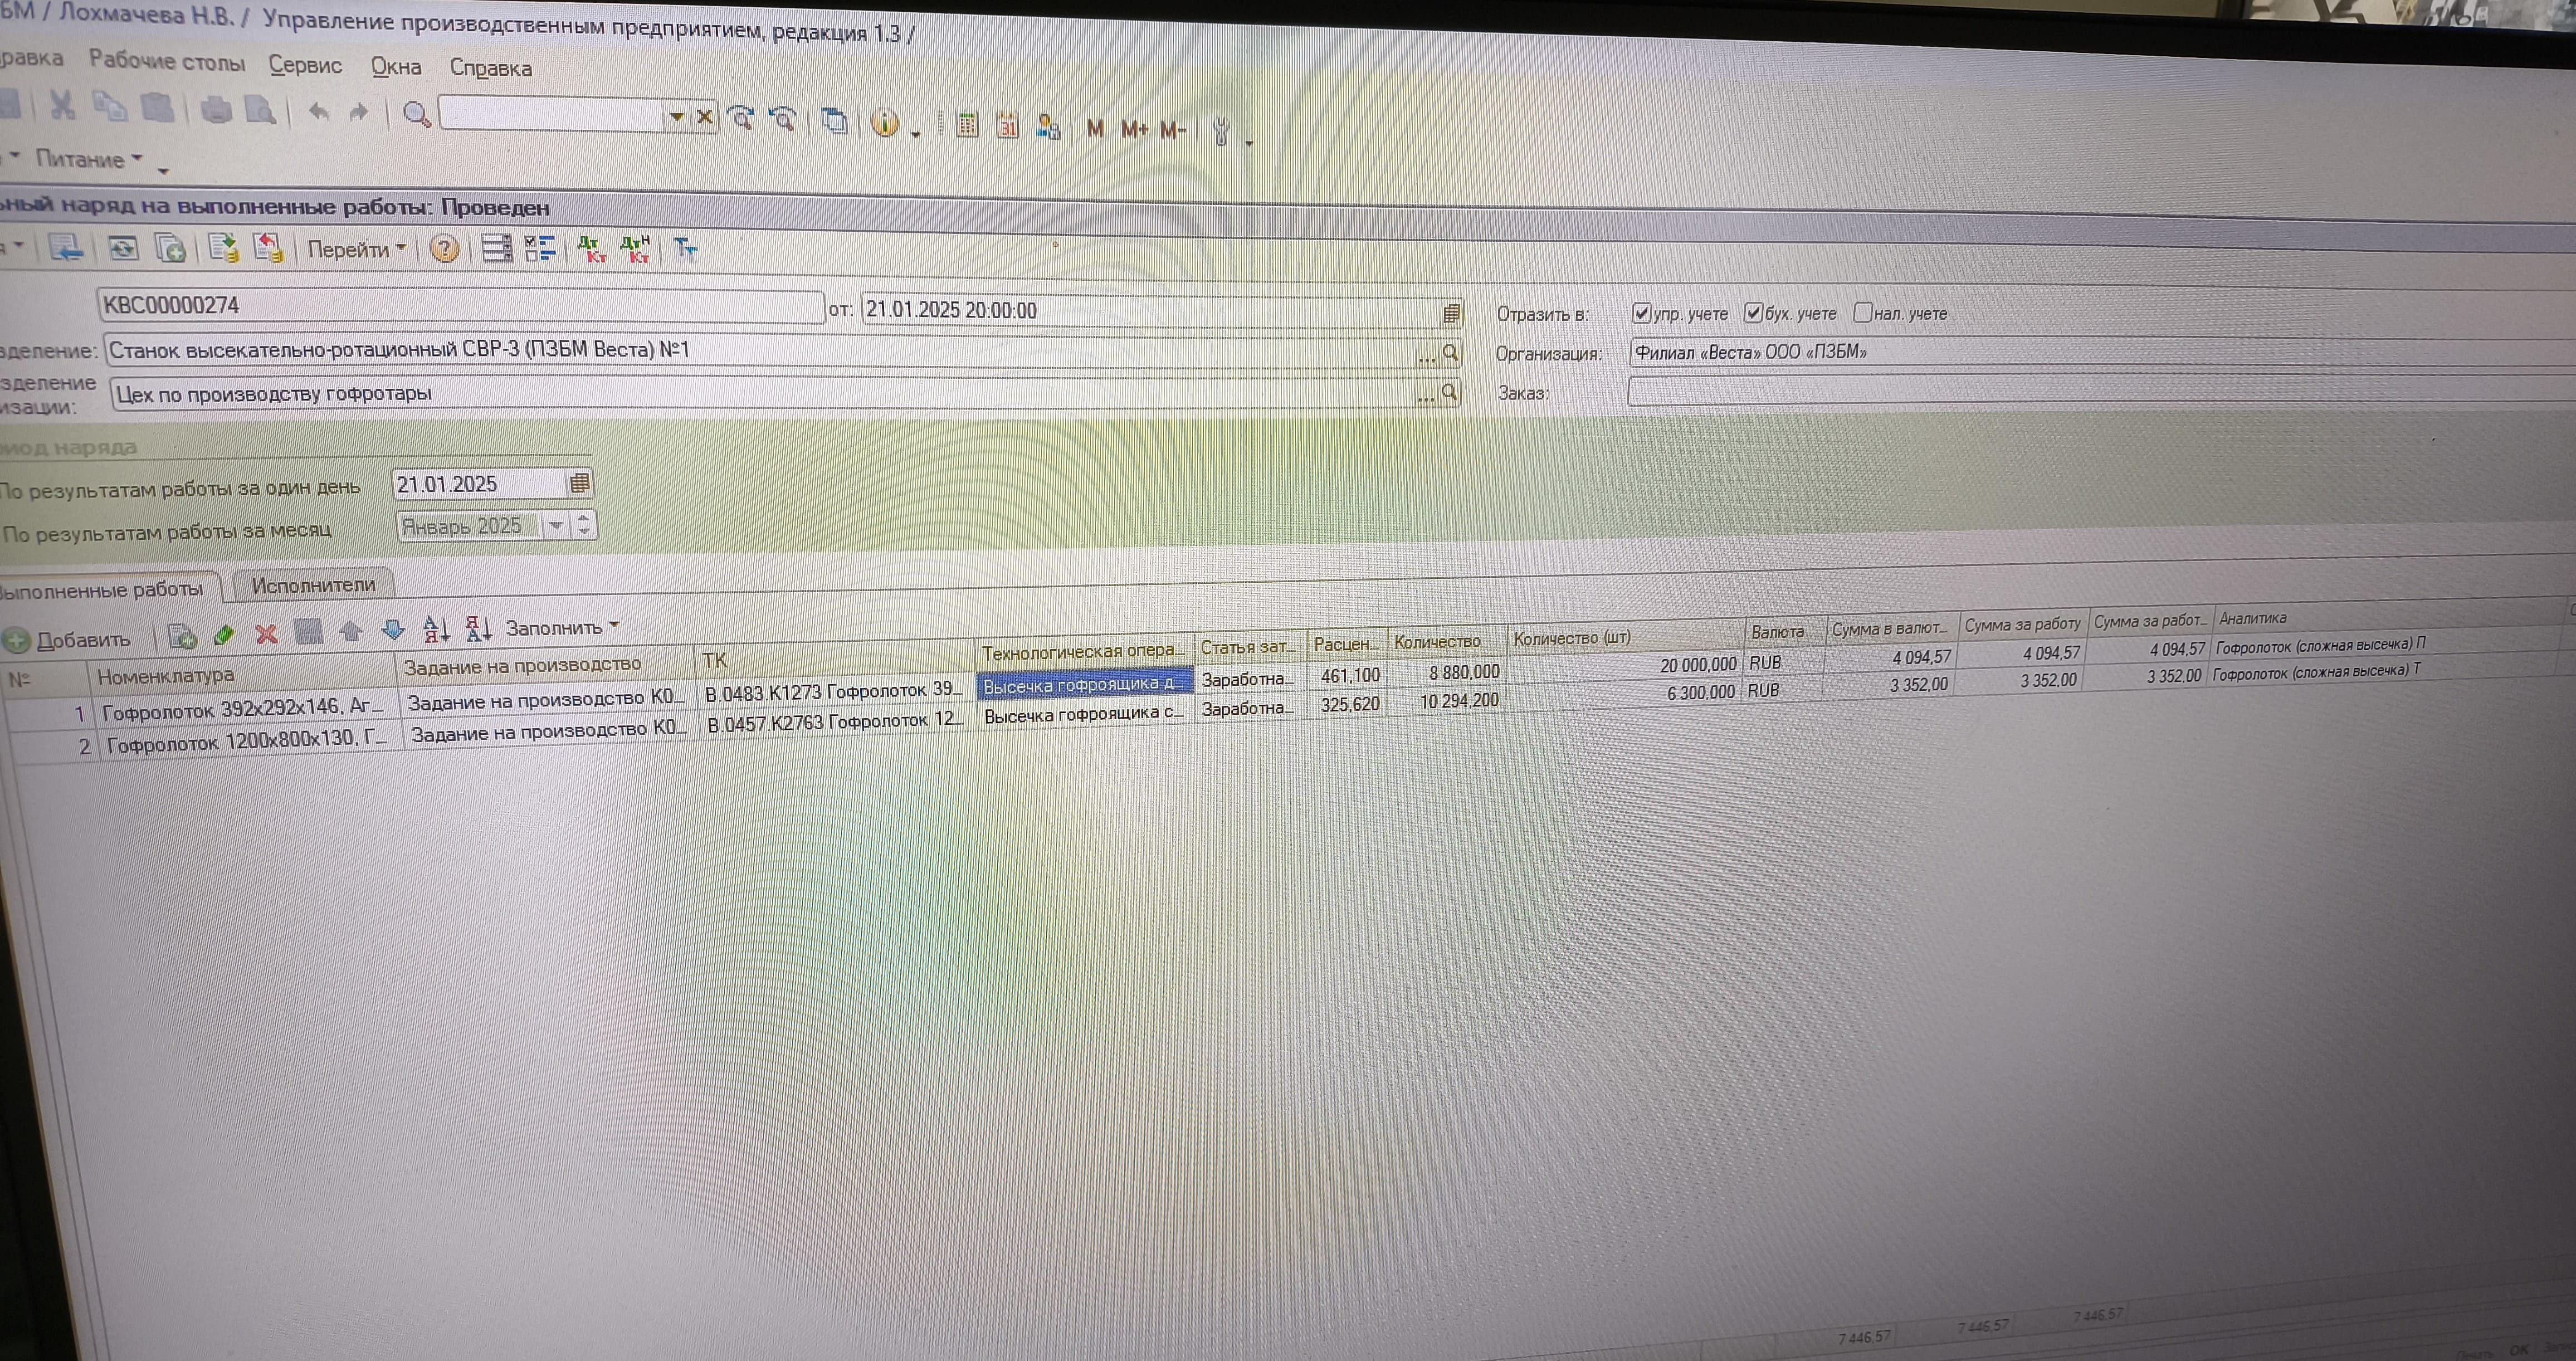
\includegraphics[height=0.35\textheight, keepaspectratio]{Pics/IIIсдельныйнаряд.jpg}
%\end{center}
 %\caption{Сдельные наряды}
 %\label{pic:IIIсдельныйнаряд}
%\end{figure}
% \begin{figure}
% \begin{center}
%   \includegraphics[height=0.4\textheight, angle=90, keepaspectratio]{Pics/f44.jpg}
% \end{center}
%   \caption{Табель учета рабочего времени}
%   \label{pic:f44}
% \end{figure}
\ifx \notincludehead\undefined
\normalsize
\end{document}
\fi
\clearpage